\documentclass{article} % For LaTeX2e
\usepackage{nips15submit_e,times}
\usepackage{hyperref}
\usepackage{url}
\usepackage{times}
\usepackage{epsfig}
\usepackage{graphicx}
\usepackage[labelfont=bf]{caption}
\usepackage{tabularx}
\usepackage{amsmath}
\usepackage{amssymb}
%\documentstyle[nips14submit_09,times,art10]{article} % For LaTeX 2.09


\title{You Only Look Once: Unified, Real-Time Object Detection}


\author{Joseph Redmon\\
University of Washington\\
\texttt{pjreddie@cs.washington.edu}
% For a paper whose authors are all at the same institution,
% omit the following lines up until the closing ``}''.
% Additional authors and addresses can be added with ``\and'',
% just like the second author.
% To save space, use either the email address or home page, not both
\and
Santosh Divvala\\
Allen Institute for Artificial Intelligence\\
\texttt{santoshd@allenai.org}
\and
Ross Girshick\\
Microsoft Research\\
\texttt{rbg@microsoft.com}
\and
Ali Farhadi\\
University of Washington\\
\texttt{ali@cs.washington.edu}
}

% The \author macro works with any number of authors. There are two commands
% used to separate the names and addresses of multiple authors: \And and \AND.
%
% Using \And between authors leaves it to \LaTeX{} to determine where to break
% the lines. Using \AND forces a linebreak at that point. So, if \LaTeX{}
% puts 3 of 4 authors names on the first line, and the last on the second
% line, try using \AND instead of \And before the third author name.

\newcommand{\fix}{\marginpar{FIX}}
\newcommand{\new}{\marginpar{NEW}}

%\nipsfinalcopy % Uncomment for camera-ready version

\begin{document}


\maketitle

\begin{abstract}
We present unified system for object detection. Our system processes images in real-time at 45 frames per second, and achieves 53.5\% mean average precision on the \textsc{Pascal} VOC object detection benchmark. A single neural network predicts bounding boxes and class probabilities directly from full images. Notably, our system does not rely on pre-processing, region proposals, sliding window techniques, or post-processing of bounding boxes. Due to this simplicity, our system runs hundreds to thousands of times faster than comparable detection systems like DPM or R-CNN.
\end{abstract}

\section{Introduction}

Humans glance at an image and instantly know what objects are in the image, where they are, and how they interact. Our fast, accurate visual system allows us to perform complex tasks like driving or grocery shopping with little conscious thought. Fast, accurate, computational object detection would allow computers to drive cars in any weather without specialized sensors, enable assistive devices to convey real-time scene information to human users, and unlock the potential for general purpose, responsive robotic systems.

Convolutional neural networks (CNNs) achieve human-level performance on classification tasks at super-human speeds. Yet the best object detection systems stare at images for tens of seconds and still make stupid mistakes. These shortcomings directly result from how these systems approach object detection.

Current systems repurpose classifiers to perform detection. To detect an object these systems take a classifier for that object and evaluate it at various locations and scales in a test image. Systems like deformable parts models (DPM) use a sliding window approach where the classifier is run at evenly spaced locations over the entire image. More recent approaches use region proposal methods to first generate potential bounding boxes in an image and then run the classifier on these proposed boxes. After classification, post-processing is used to refine the bounding box, eliminate duplicate or overlapping detections, and rescore the box based on other objects in the scene.

\begin{figure}[t]
\begin{center}
        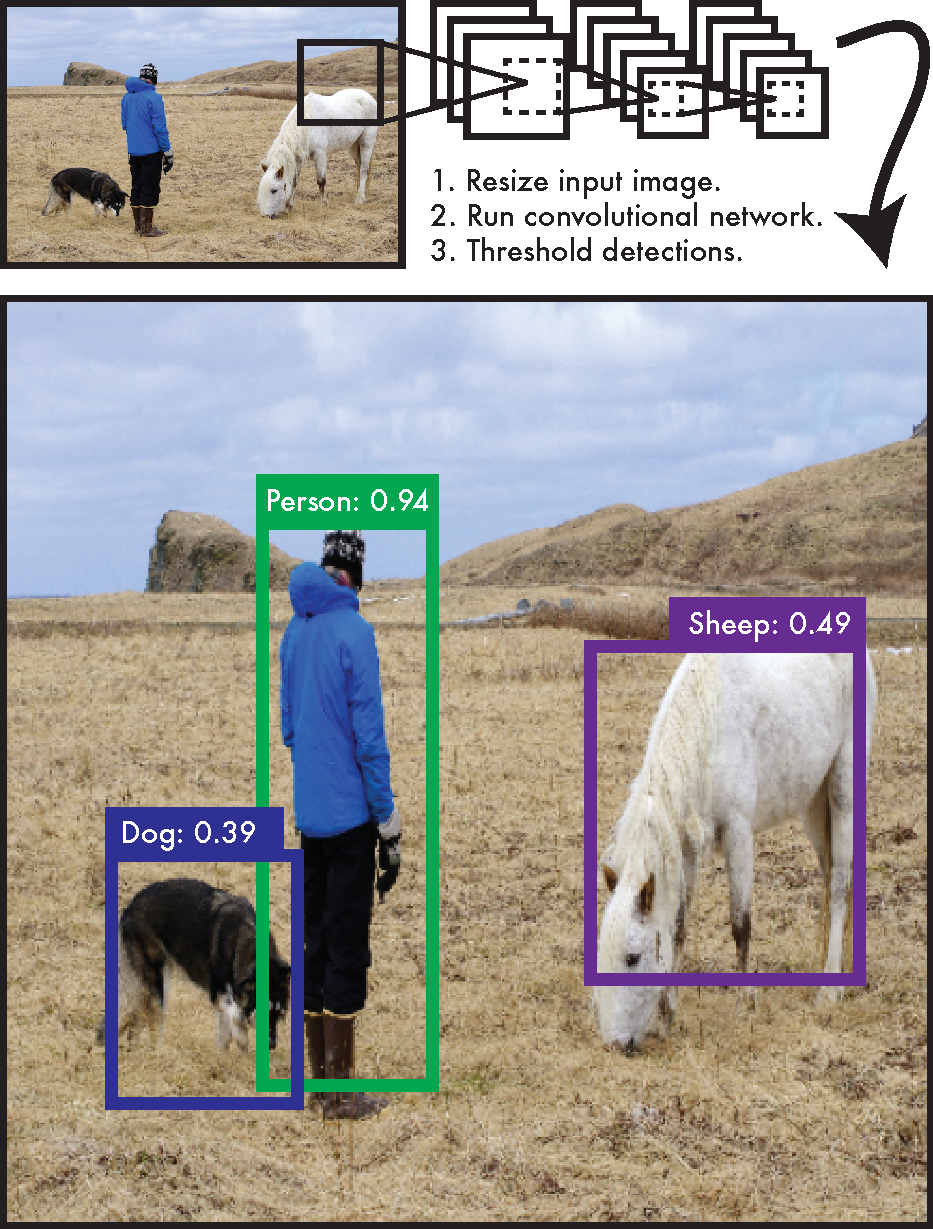
\includegraphics[width=.4\linewidth]{system}
\end{center}
   \caption{\textbf{The YOLO Detection System.} Our system (1) resizes the input image to $448 \times 448$, (2) runs a single convolutional network on the image, and (3) thresholds the resulting detections by the model's confidence. For all examples in this paper we use a confidence threshold of $0.2$ unless otherwise noted.}
\label{system}
\end{figure}

These region proposal techniques typically generate between a few hundred and a few thousand potential boxes per image. Selective Search, the most common region proposal method, takes 1-2 seconds per image to even generate the potential boxes. The classifier then takes additional time to evaluate each of these potentially thousands of proposals. The best performing systems require 10-20 seconds per image while even those optimized for speed come no where close to real-time performance.

Additionally, even a highly accurate classifier will produce false positives when faced with so many proposals. Detection systems use non-maximal suppression and other post-processing techniques to mitigate these false positives but that introduces other problems. For example, non-maximal suppression makes it difficult to detect two objects of the same class that overlap by a significant margin. Due to these inherent limitations, even state-of-the-art detection systems make obvious mistakes on test images.

Finally, these detection pipelines rely on independent techniques at every stage that cannot be optimized jointly. A typical pipeline uses Selective Search for region proposals, a convolutional network for feature extraction, a collection of one-versus-all SVMs for classification, non-maximal suppression to reduce duplicates, and a linear model to adjust the final bounding box coordinates. Selective Search tries to maximize recall while the SVMs optimize for single class accuracy and the linear model learns from localization error.

Our system is refreshingly simple. A single convolutional network simultaneously predicts multiple bounding boxes and class probabilities for those boxes. Our system enforces spatial diversity in the proposed bounding boxes without relying on non-maximal suppresion to eliminate deplicates. We train our network on full images to directly optimize detection performance. At test time, a single network evalution produces complete detections without any pre or post-processing.

\section{Unified Detection}

Redmon et al. use a single convolutional network to perform robotic grasp detection \cite{DBLP:journals/corr/RedmonA14}. Their MultiGrasp system simultaneously predicts potential grasping rectangles for an object and probabilities for those grasps. We generalize their approach to the problem of object detection in images.

Using our system, you only look once (YOLO) at an image to predict what objects are present and where they are. The YOLO design enables end-to-end training and real-time speeds while maintaining high average precision.

\subsection{Design}

\begin{figure}[t]
\begin{center}
        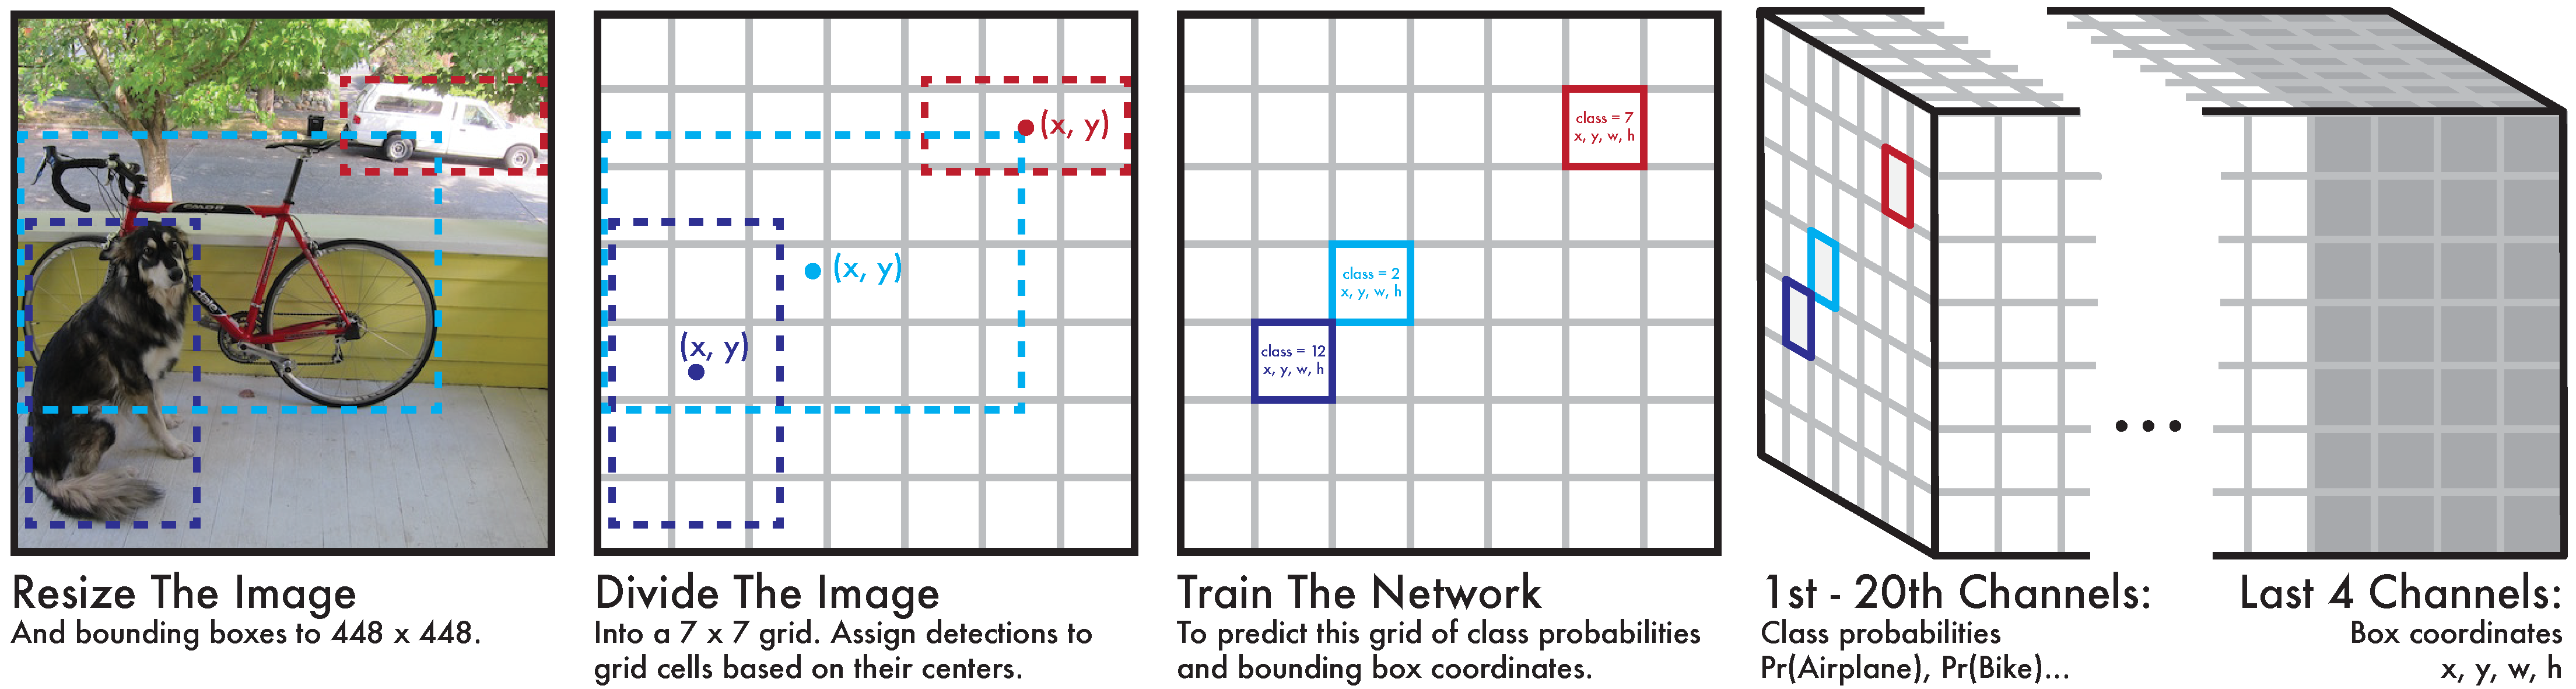
\includegraphics[width=\linewidth]{full}
\end{center}
   \caption{\textbf{The Model.} Our system models detection as a regression problem to a $7 \times 7 \times 24$ tensor. This tensor encodes bounding boxes and class probabilities for objects in the image.}
\label{model}
\end{figure}


Our system divides the image into a $7 \times 7$ grid. If the center of an object falls into a grid cell, that grid cell is responsible for detecting that object. Each grid cell predicts a bounding box and class probabilities associated with that bounding box.

We implement this model as a convolutional neural network for use on the \textsc{Pascal} VOC detection dataset \cite{Everingham15}. The initial convolutional layers of the network extract features from the image while the fully connected layers predict the output probabilities and coordinates.

Our network architecture is inspired by the GoogLeNet model for image classification \cite{DBLP:journals/corr/SzegedyLJSRAEVR14}. The nework has 23 convolutional layers followed by 2 fully connected layers. However, instead of the inception modules used by GoogLeNet we simply use $1 \times 1$ reduction layers followed by $3 \times 3$ convolutional layers. We also replace maxpooling layers with strided convolutions.

The final output of our network is a $7 \times 7$ grid of predictions. Each grid cell predicts 20 conditional class probabilities, and 4 bounding box coordinates.

   \begin{figure}[h]
      \centering
        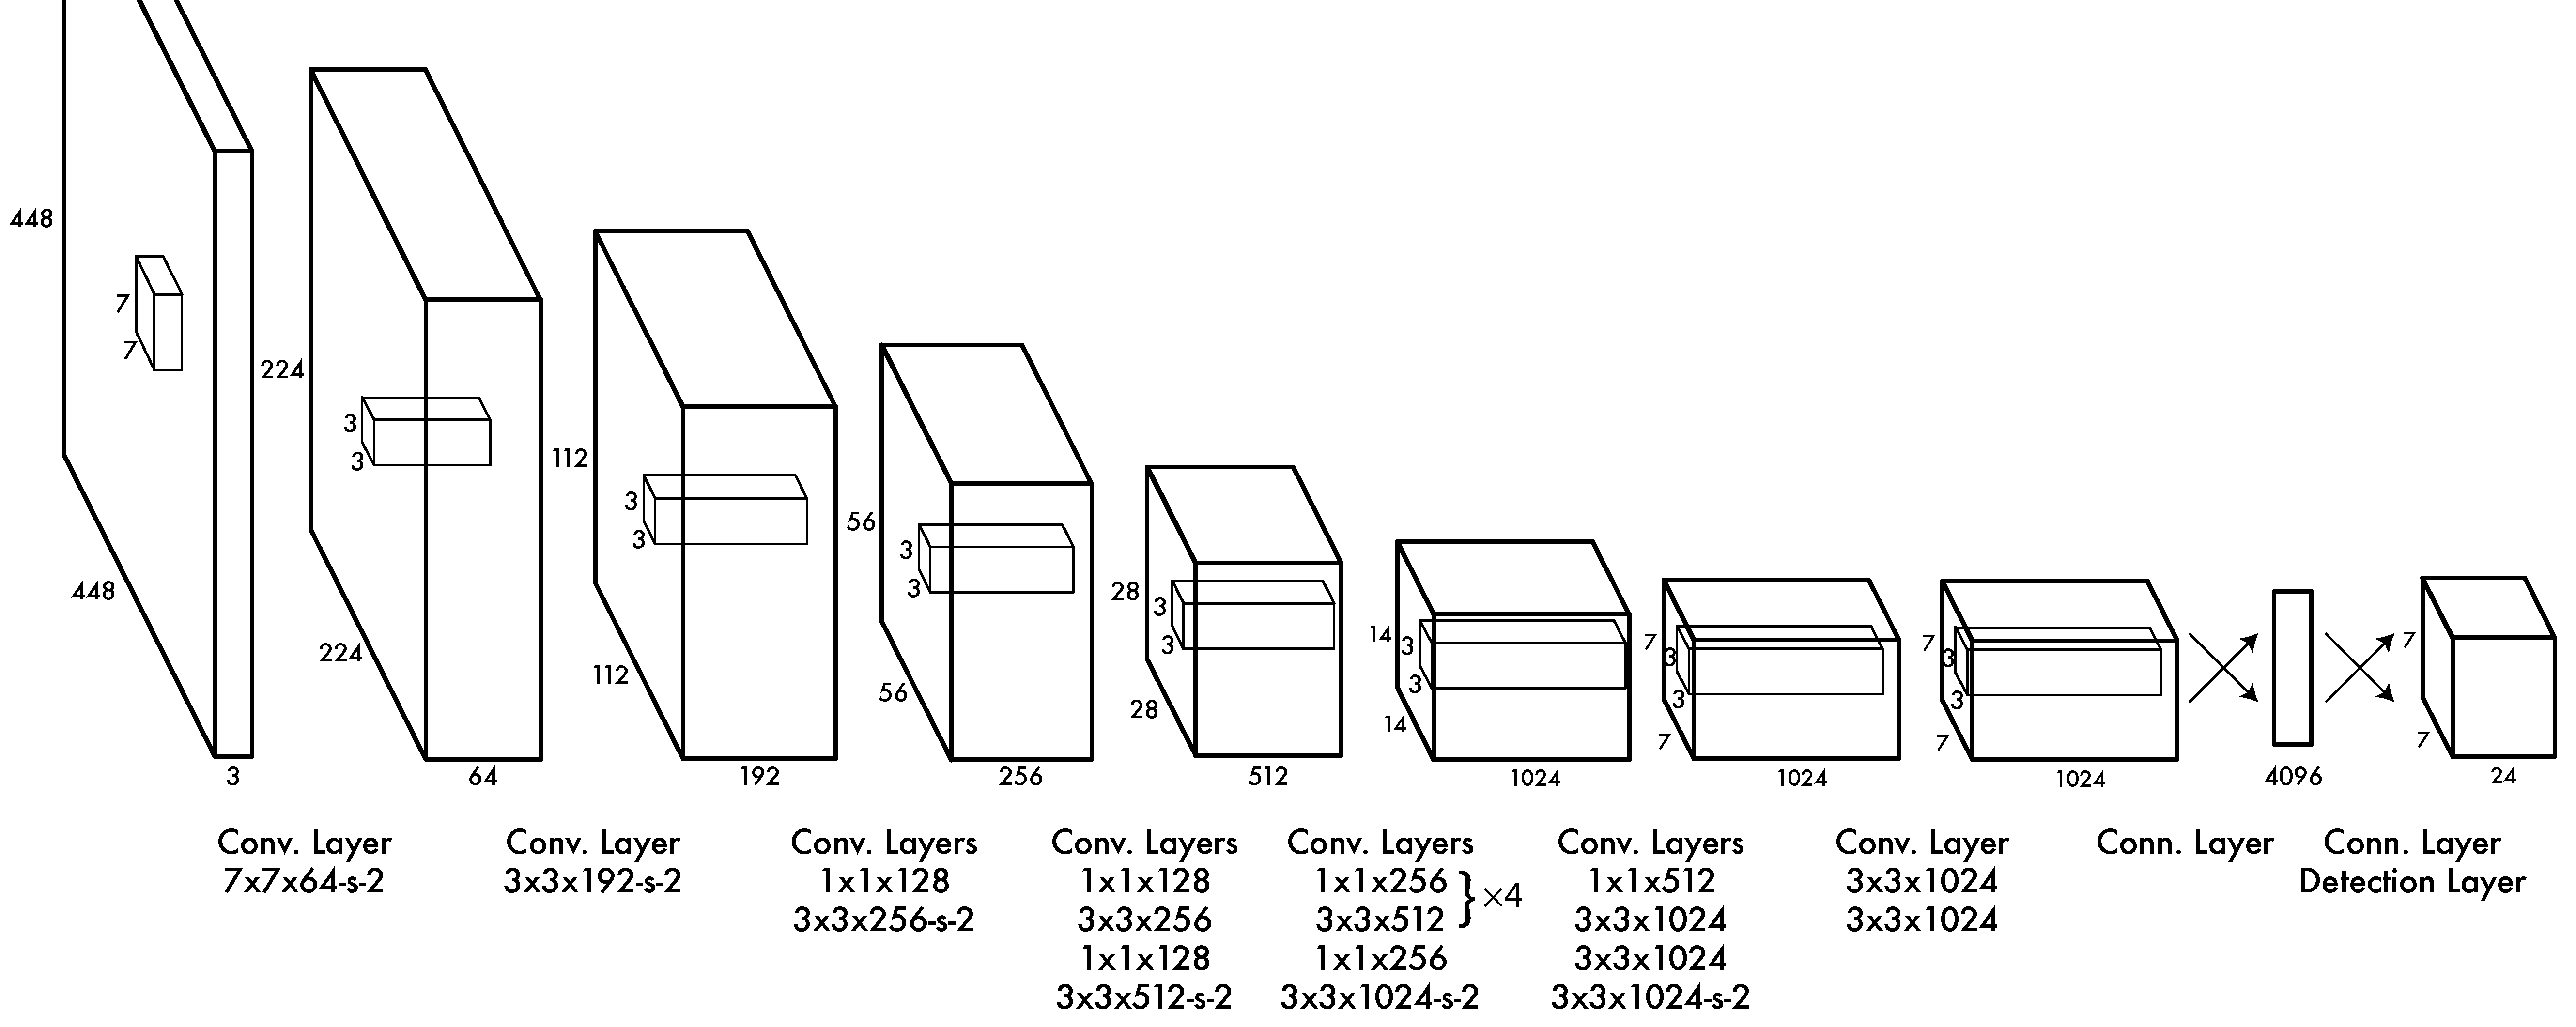
\includegraphics[width=\linewidth]{detectnet2}
      \caption{\textbf{The Architecture.} Our detection network has 23 convolutional layers followed by 2 fully connected layers. The network uses strided convolutional layers to downsample the feature space instead of maxpooling layers. Alternating $1 \times 1$ convolutional layers reduce the features space from preceeding layers. We pretrain the convolutional layers on the ImageNet classification task at half the resolution ($224 \times 224$ input image) and then double the resolution for detection.}
      \label{net}
   \end{figure}


\subsection{Benefits and Limitations}

\begin{figure}[th]
\begin{center}
        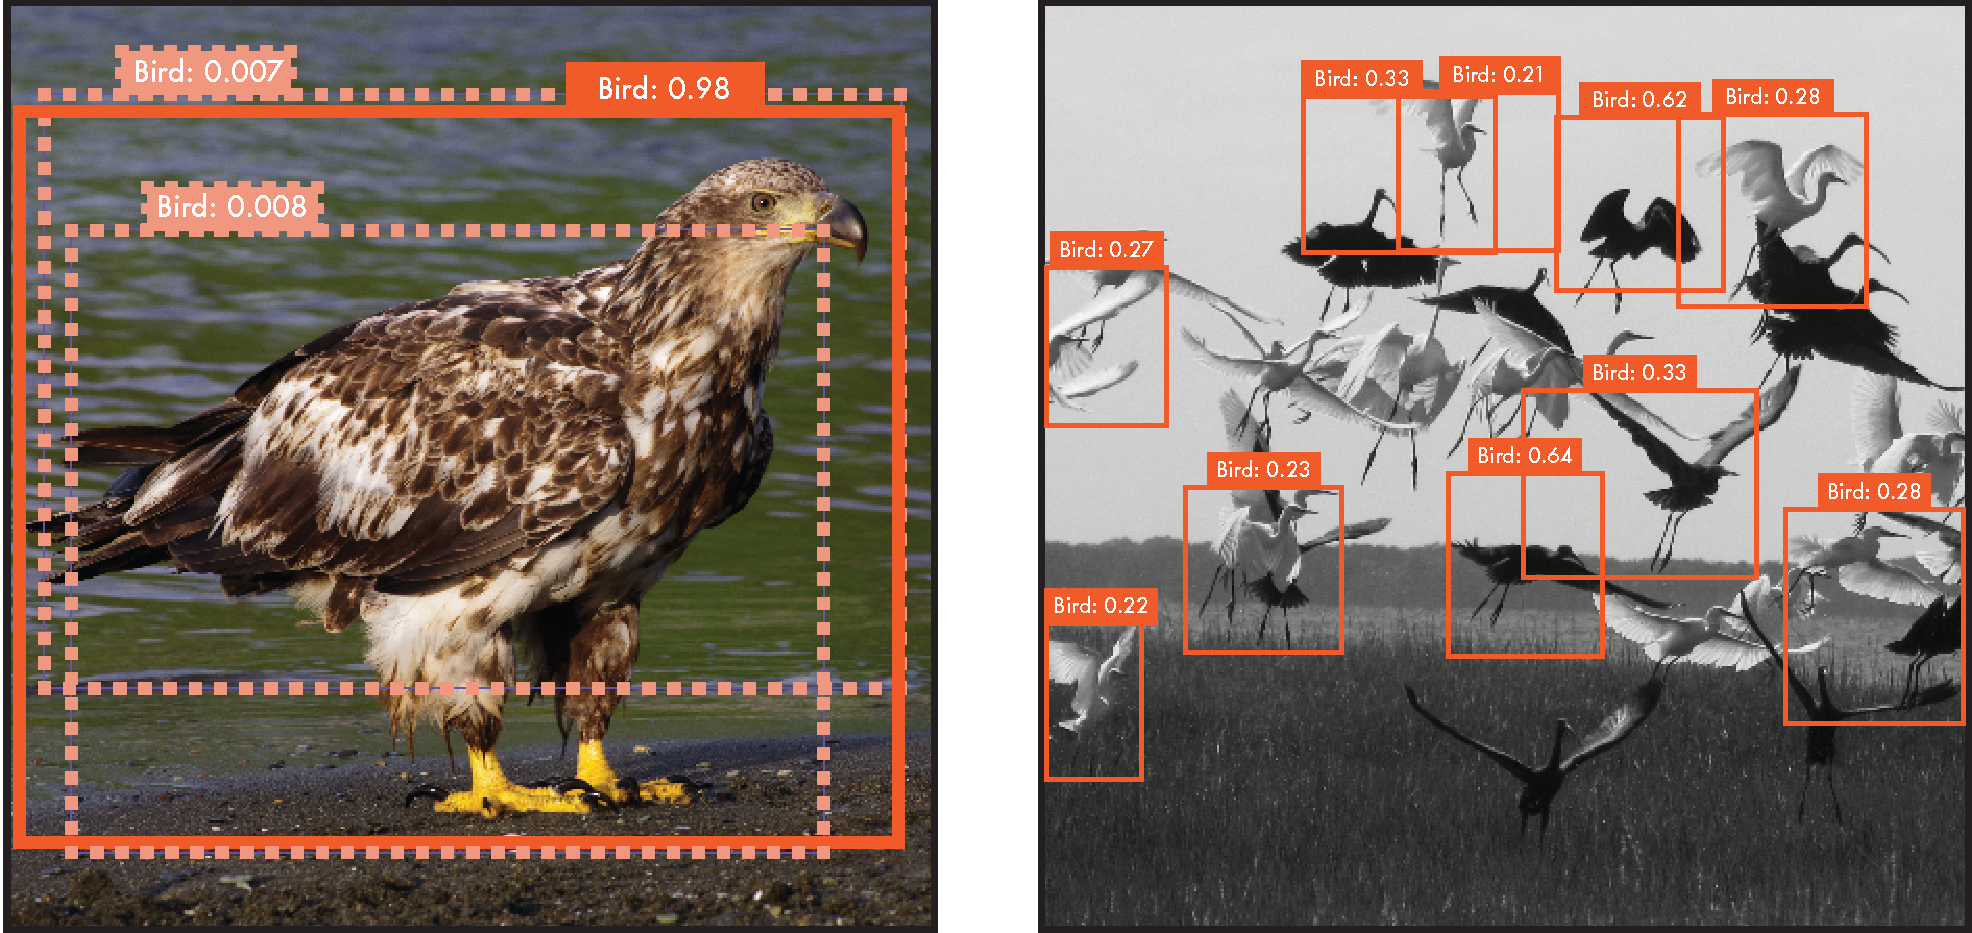
\includegraphics[width=.8\linewidth]{bird}
\end{center}
   \caption{\textbf{No NMS needed.} Our model makes local predictions but it reasons about the entire image. When multiple grid cells can predict good bounding boxes for an object, the model picks the best cell and downweights surrounding predictions. \textbf{Problems with small objects in groups.} The spatial constraint we impose restricts the model's ability to predict boxes for multiple small objects that are next to each other in an image. Our model cannot predict correct bounding boxes for multiple objects if they fall into the same grid cell.}
\label{eagle}
\end{figure}

This model and architecture form a unified pipeline for object detection. It is simple to construct and can be trained directly on full images to optimize for detection performance. Moreover, it predicts detections with only a single network evaluation, making it extremely fast.

A cell is only responsible for objects centered in that cell so we restrict the coordinates to fall within that cell. This imposes a strong spatial constraint on the predictions which has both benefits and drawbacks. Cells rarely predict multiple bounding boxes for the same object in an image which eliminates the need for non-maximal supression or other post-processing.

Conversely, this spatial constraint limits the number of nearby objects that our model can predict. If two objects fall into the same cell our model can only predict one of them. Our model struggles with small objects that appear in groups, such as flocks of birds.

While this limits our performance on benchmarks like \textsc{Pascal}, it also mimics how humans visually percieve objects. Humans quickly count small numbers of objects ($N \le 4$) but take significantly more time per object to count larger groups of objects \cite{piazza2002subitizing}. This suggests that the human visual system can natively handle a small number of objects but after some threshold we require additional post-processing.

\subsection{Comparison to Deformable Parts Models}

Deformable parts models (DPM) epitomize the sliding window approach to object detection \cite{lsvm-pami}. DPM first extracts features from an image (usually Histogram of Oriented Gradients), then runs classifiers (object templates) over every location in the feature space. DPM relies on static image features and uses SVMs to classify image patches. These SVMs independently learn to classify patches and typically only see small amounts of local context.

After the initial classification, high scoring detections undergo significant post-processing. First, a linear model predicts the actual bounding box from the filter filter locations and scores. Then non-maximal supression eliminates duplicate detections. Finally, specially trained SVMs rescore the detection.

Our system replaces all of these disparate parts with a single convolutional neural network. The network performs feature extraction, bounding box prediction, non-maximal suppression, and contextual reasoning all concurrently. Instead of static features, the network trains the features in-line and optimizes them for the detection task. Our unified architecture leads to a faster, more accurate model than DPM.

The convolutional layers of our architecture do bare some similarity to DPM. Convolutional layers run filters over every location on an input feature map. Some filters in our model likely function as part templates or whole object templates. However, unlike DPM, these filters are only an intermediate step in our full model. The fully connected layers take the filter responses and reason globally about objects in the image. Our essentially brings together each of the separate pieces from DPM and optimizes them jointly.

\subsection{Comparison to Region Proposal Methods}

Another class of detection algorithms uses region proposals instead of sliding windows to find objects in images. These systems use region proposal methods like Selective Search \cite{uijlings2013selective} to generate potential bounding boxes in an image. Instead of scanning through every region in the window, now the classifier only has to score a small subset of potential regions in an image. Good region proposal methods maintain high recall despite greatly limiting the search space.

Selective Search in its most common setting ("fast mode") generates around 2,000 regions per image. Compared to DPM this is about a 100-fold reduction in the number of regions a detection system evaluates. This reduction allows detection systems to use more accurate but computationally complex classifiers on the proposed regions.

The most widely used system, R-CNN, uses a convolutional neural network to extract features from the regions and then SVMs to classify them \cite{girshick2014rich}. R-CNN shares many design aspects with DPM. After region proposal, R-CNN uses the same multi-stage pipeline of feature extraction (using CNNs instead of HOG), SVM scoring, non-maximal suppression, and bounding box prediction using a linear model.

Though similar, R-CNN outperforms DPM by a wide margin. Instead of using static HOG features, R-CNN uses convolutional features finetuned for a given dataset. Due to Selective Search, R-CNN sees fewer regions in an image than DPM and is less susceptible to false positives.

This performance comes at a cost. Selective Search, even in "fast mode" takes about 2 seconds to propose regions for an image. Moreover, convolutional features take time to compute, especially for 2000 independent regions. The best performing R-CNN method with post-processing takes about 40 seconds per image \cite{DBLP:journals/corr/ZhuUSF15}. Recent work to speed up R-CNN uses a faster region proposal method (Edge Boxes \cite{zitnick2014edge}) and feature sharing between regions for much higher throughput but also lower average precision \cite{he2014spatial}.

YOLO shares some similarities with R-CNN. Each grid cell proposes a potential bounding box and then scores that bounding box using convolutional features. However, our system puts spatial constraints on the grid cell proposals which helps mitigate multiple detections of the same object. Our system also proposes far fewer bounding boxes, only 49 per image compared to about 2000. Finally, our system combines these individual components into a single, jointly optimized model.

\subsection{Comparison to DeepMultiBox}

Most R-CNN variants use Selective Search to generate region proposals. Szegedy et al. instead train a convolutional neural network to predict regions of interest \cite{erhan2014scalable}. They cluster ground truth bounding boxes into 800 groups and then given an image, predict confidence scores for each of these 800 clusters. They threshold the predicted bounding boxes so that before classification most are thrown out.

MultiBox performs similarly to Selective Search but with fewer region proposals. Fewer proposals leads to less work during classification and a large boost in throughput. MultiBox can also perform single object detection by replacing the confidence prediction with a single class prediction. However, MultiBox cannot perform general object detection and is still just a piece in a larger detection pipeline.

Both YOLO and MultiBox use a convolutional network to predict bounding boxes and confidence scores. However, YOLO additionally predicts class-specific probabilities making it able to perform general object detection. Instead of predicting bounding boxes based on clusters, YOLO uses the grid approach to enforce spatial diversity in predicted clusters. MultiBox relies on non-maximal suppression and post-processing which YOLO does not need.

\subsection{Comparison to OverFeat}

Sermanet et al. train a convolutional neural network to perform localization and adapt that localizer to perform detection \cite{DBLP:journals/corr/SermanetEZMFL13}. Overfeat represents the localizer as a convolutional layer in the network and applies it in a sliding window fashion to the image at multiple locations and scales. Overfeat then merges the resulting localization boxes into discrete detections.

Overfeat efficiently performs sliding window detection but it is still a disjoint system. Overfeat optimizes for localization, not detection performance. Like DPM, the localizer only sees local information when making a prediction. Overfeat cannot reason about global context and thus requires significant post-processing to produce coherent detections.

\section{Training}

   \begin{figure*}[t]
      \centering
        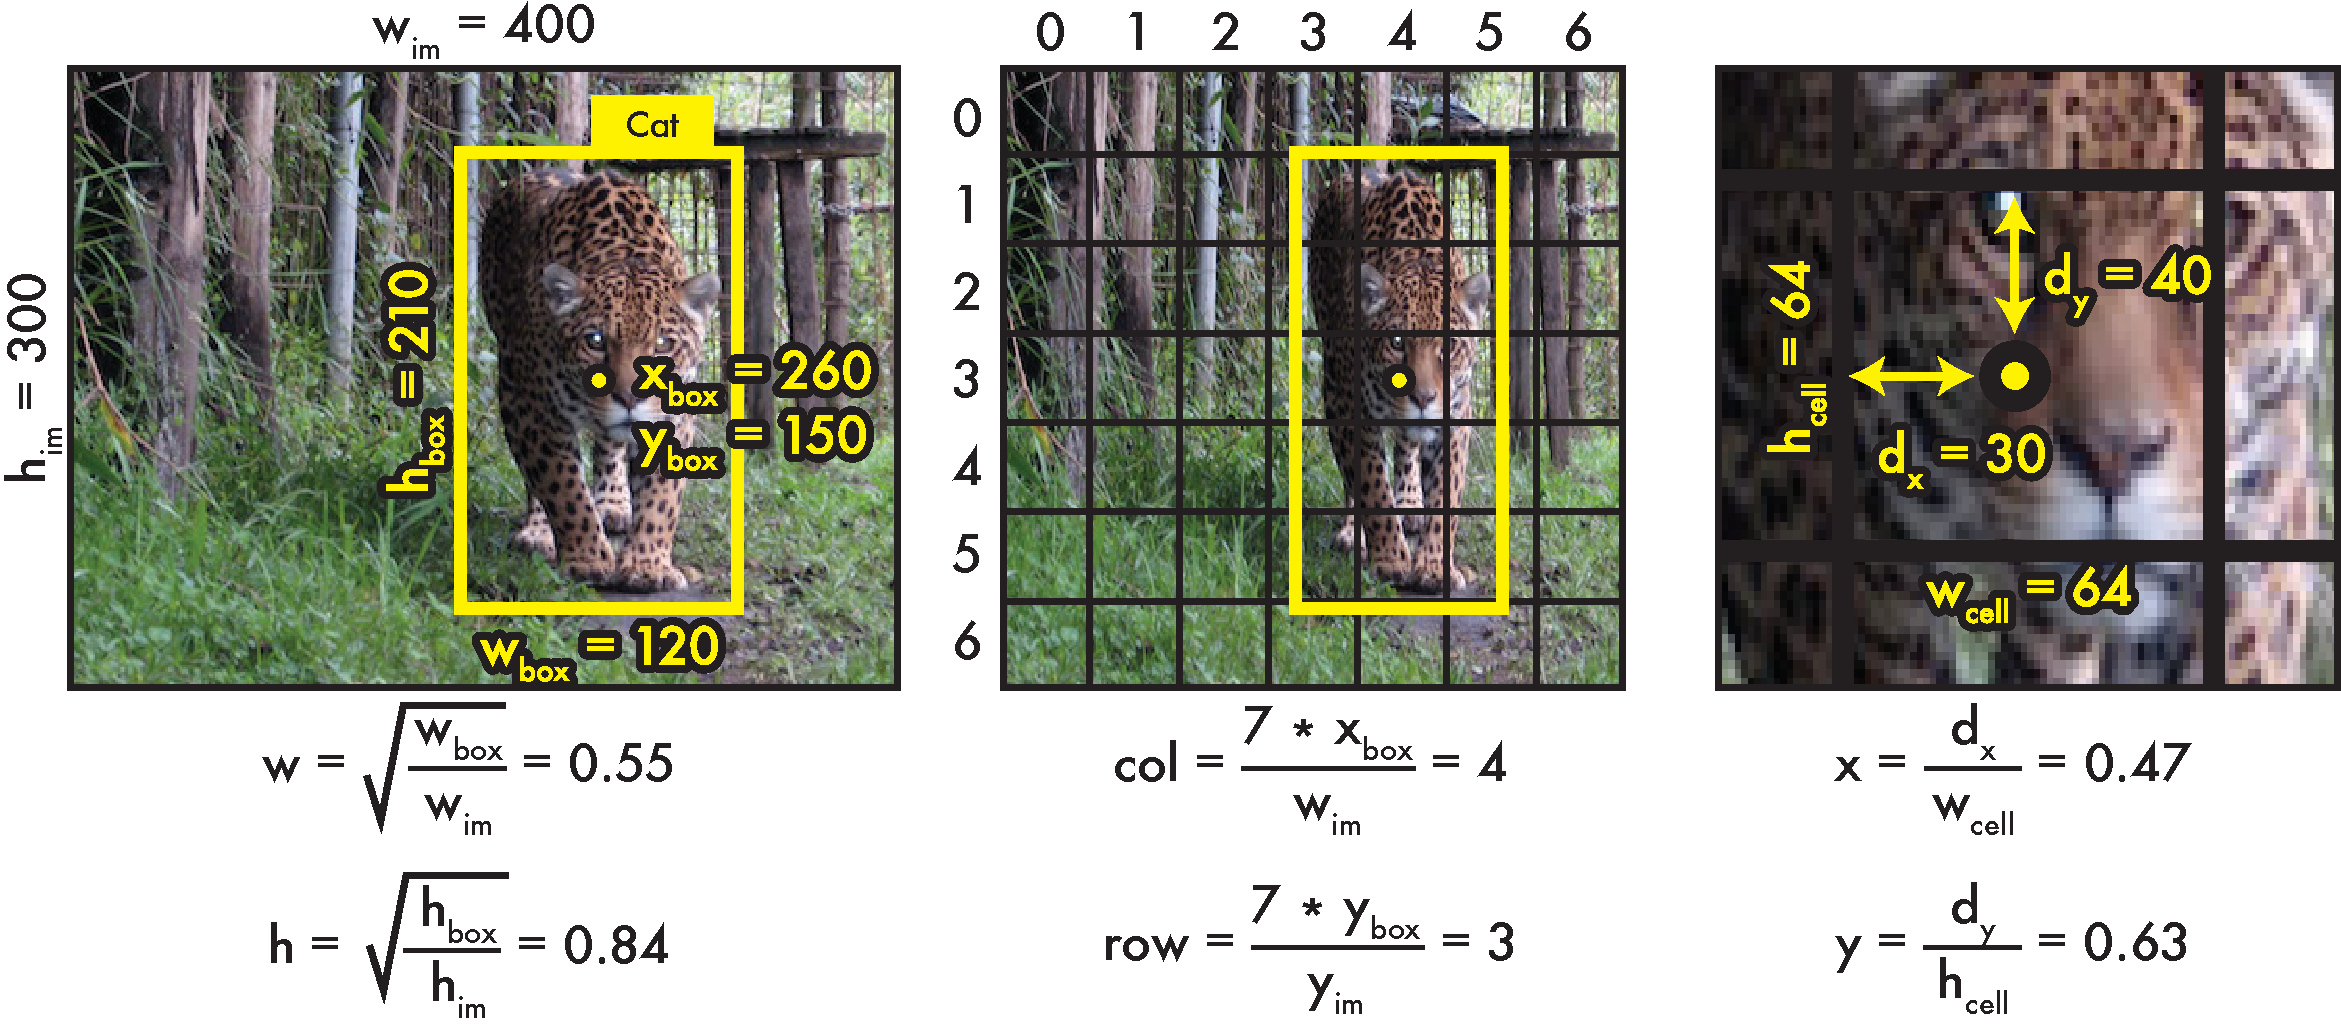
\includegraphics[width=.8\linewidth]{transform}
      \caption{\textbf{The Coordinate System.} This image shows an example transformation from bounding box coordinates to the coordinates used by our output layer.}
      \label{transform}
   \end{figure*}

We pretrain our convolutional layers on the ImageNet 1000-class competition dataset \cite{ILSVRC15}. For pretraining we use the first 20 convolutional layers from \ref{net} followed by a maxpooling layer and two fully connected layers. We train this network for approximately a week and achieve top-5 accuracy of 86\% on the ImageNet 2012 validation set.

We then adapt the model to perform detection. We add three convolutional layers and two fully connected layers with randomly initialized weights. Detection often requires fine-grained visual information so we increase the input resolution of the network from $224 \times 224$ to $448 \times 448$.

Our final layer predicts both class probabilities and bounding box coordinates. We normalize the bounding box width and height by the image width and height so that they fall between 0 and 1. We parameterize the bounding box $x$ and $y$ coordinates to be offsets of a particular grid cell location so they are also bounded between 0 and 1. We use a logistic activation function to reflect these constraints on the final layer. All other layers use the following leaky rectified linear activation:

\begin{equation}
\phi(x) =
\begin{cases}
    1.1x, & \text{if } x > 0\\
    .1x, & \text{otherwise}
    \end{cases}
\end{equation}

We optimize for sum-squared error in the output of our model. We chose sum-squared error because it is easy to optimize however it does not perfectly align with our actual goal of maximizing average precision. It weights localization error equally with classification error which may not be ideal. To remedy this, we use a scaling factor to adjust weight given to error from coordinate predictions versus error from class probabilities. In our final model we use a scaling factor of 4.

Sum-squared error also equally weights errors in large boxes and small boxes. Our error metric should reflect that small deviations in large boxes matter less than in small boxes. To partially address this we predict the square root of the bounding box width and height instead of the width and height directly.

We train the network for about 100 epochs on the training and validation data sets from \textsc{Pascal} VOC 2007 and 2012 as well as the test set from 2007, a total of 21k images. Throughout training we use a batch size of 64, a momentum of $0.9$ and a decay of $0.0005$. We use two learning rates during training: $10^{-2}$ and $10^{-3}$. Training diverges if we use the higher learning rate, $10^{-2}$, from the start. We use the lower rate, $10^{-3}$, for one epoch so that the randomly initialized weights in the final layers can settle to a reasonable value. Then we train with the following learning rate schedule: $10^{-2}$ for 60 epochs, and $10^{-3}$ for 30 epochs.

\subsection{Nuisance Variables}

Each grid cell predicts class probabilities for that area of the image. There are 49 cells with a possible 20 classes each yielding 980 predicted probabilities per image. Most of these will be probabilities will be zero since only a few obejects appear in any given image. Left unchecked, this imbalance pushes all of the probabilities to zero, leading to divergence during training.

To overcome this, we add an extra variable to each grid location, the probability that any object exists in that location regardless of class. Thus instead of 20 class probabilities we have 1 "objectness" probability, $\Pr(\textrm{Object})$, and 20 conditional probabilities: $\Pr(\textrm{Airplane | Object})$, $\Pr(\textrm{Bicycle | Object})$, etc.

To get the unnormalized probability for an object class at a given location we simply multiply the "objectness" probability by the conditional class probability:

\begin{equation}
\Pr(\textrm{Cat}) = \Pr(\textrm{Object}) * \Pr(\textrm{Cat} | \textrm{Object})
\end{equation}

We can optimize these probabilities independently or jointly using a novel "detection layer" in our convolutional network. During the initial stages of training we optimize them independently to improve model stability. We update the "objectness" probabilities at every location however we only update the conditional probabilities at locations that actually contain an object. This means there are far fewer probabilities getting pushed towards zero. 

During later stages of training we optimize the unconditioned probabilities by performing the required multiplications in the network and calculating error based on the result.

\section{Evaluation}

We evaluate YOLO on the test sets for \textsc{Pascal} VOC 2010 and 2012. 

\begin{table*}
\tiny
\newcolumntype{Y}{>{\centering\arraybackslash}X}
\begin{center}
\tabcolsep=0.11cm
\begin{tabularx}{\linewidth}{@{}l|Y|Y Y Y Y Y Y Y Y Y Y Y Y Y Y Y Y Y Y Y Y}
\textbf{VOC 2012 test} & mAP & aero & bike & bird & boat & bottle & bus & car & cat & chair & cow & table & dog & horse & mbike & person & plant & sheep & sofa & train & tv \\
\hline
MR\_CNN\_S\_CNN & 70.7& 85.0& 79.6& 71.5& 55.3& 57.7& 76.0& 73.9& 84.6& 50.5& 74.3& 61.7& 85.5& 79.9& 81.7& 76.4& 41.0& 69.0& 61.2& 77.7& 72.1 \\
DEEP\_ENS\_COCO &  70.1& 84.0& 79.4& 71.6& 51.9& 51.1& 74.1& 72.1& 88.6& 48.3& 73.4& 57.8& 86.1& 80.0& 80.7& 70.4& 46.6& 69.6& 68.8& 75.9& 71.4 \\
\textbf{Fast R-CNN + YOLO} & 70.0 & 83.0 & 78.4 & 73.4 & 55.7 & 42.5 & 78.2 & 72.7 & 89.5 & 48.2 & 74.0 & 56.4 & 87.2 & 80.8 & 80.7 & 74.4 & 41.1 & 70.0 & 67.1 & 71.2 & 66.0 \\
Nets on Conv. Feats. &68.8& 82.8& 79.0& 71.6& 52.3& 53.7& 74.1& 69.0& 84.9& 46.9& 74.3& 53.1& 85.0& 81.3& 79.5& 72.2& 38.9& 72.4& 59.5& 76.7& 68.1\\
NUS\_NIN\_C2000 & 63.8 & 80.2 & 73.8 &  61.9 &  43.7 &  43.0 &  70.3 &  67.6 &  80.7 &  41.9 &  69.7 &  51.7 &  78.2 &  75.2 &  76.9 &  65.1 &  38.6 &  68.3 &  58.0 &  68.7 &  63.3 \\
BabyLearning &  63.2 &  78.0 &  74.2 &  61.3 &  45.7 &  42.7 &  68.2 &  66.8 &  80.2 &  40.6 &  70.0 &  49.8 &  79.0 &  74.5 &  77.9 &  64.0 &  35.3 &  67.9 &  55.7 &  68.7 &  62.6 \\
R-CNN VGG BB &  62.4 &  79.6 &  72.7 &  61.9 &  41.2 &  41.9 &  65.9 &  66.4 &  84.6 &  38.5 &  67.2 &  46.7 &  82.0 &  74.8 &  76.0 &  65.2 &  35.6 &  65.4 &  54.2 &  67.4 &  60.3 \\
NUS\_NIN & 62.4 &  77.9 &  73.1 &  62.6 &  39.5 &  43.3 &  69.1 &  66.4 &  78.9 &  39.1 &  68.1 &  50.0 &  77.2 &  71.3 &  76.1 &  64.7 &  38.4 &  66.9 &  56.2 &  66.9 &  62.7 \\
R-CNN VGG & 59.2 &  76.8 &  70.9 &  56.6 &  37.5 &  36.9 &  62.9 &  63.6 &  81.1 &  35.7 &  64.3 &  43.9 &  80.4 &  71.6 &  74.0 &  60.0 &  30.8 &  63.4 &  52.0 &  63.5 &  58.7 \\
Feature Edit &  56.3 &  74.6 &  69.1 &  54.4 &  39.1 &  33.1 &  65.2 &  62.7 &  69.7 &  30.8 &  56.0 &  44.6 &  70.0 &  64.4 &  71.1 &  60.2 &  33.3 &  61.3 &  46.4 &  61.7 &  57.8 \\
\textbf{YOLO} & 53.6 & 71.6 & 62.2 & 55.2 & 35.9 & 23.2 & 62.4 & 53.7 & 78.1 & 34.0 & 52.9 & 38.7 & 72.2 & 67.3 & 66.3 & 62.1 & 25.5 & 50.0 & 46.9 & 67.4 & 46.3 \\
R-CNN BB &  53.3 &  71.8 &  65.8 &  52.0 &  34.1 &  32.6 &  59.6 &  60.0 &  69.8 &  27.6 &  52.0 &  41.7 &  69.6 &  61.3 &  68.3 &  57.8 &  29.6 &  57.8 &  40.9 &  59.3 &  54.1 \\
SDS & 50.7 &  69.7 &  58.4 &  48.5 &  28.3 &  28.8 &  61.3 &  57.5 &  70.8 &  24.1 &  50.7 &  35.9 &  64.9 &  59.1 &  65.8 &  57.1 &  26.0 &  58.8 &  38.6 &  58.9 &  50.7 \\
R-CNN & 49.6 & 68.1 & 63.8 & 46.1 & 29.4 & 27.9 & 56.6 & 57.0 & 65.9 & 26.5 & 48.7 & 39.5 & 66.2 & 57.3 & 65.4 & 53.2 & 26.2 & 54.5 & 38.1 & 50.6 & 51.6 \\
\end{tabularx}
\end{center}
\caption{\textbf{Results.} Ours is better.}
\end{table*}


\section{Discussion}

{\small
\bibliographystyle{ieee}
\bibliography{egbib}
}

\end{document}
